\chapter{Electron + Muon Channel}\label{sec:eMu}

\section{Event selection}\label{sec:em_selection}

%% The electron selection is identical to that described in
%% Section~\ref{sec:et_selection}.  Muons are required to have $p_{T}>
%% 10$ GeV and $\vert \eta \vert < 2.1$, with a distance of closest
%% approach to the leading sum-$p_T^2$ primary vertex of less than
%% 0.045~cm (transvese) and 0.2~cm (longitudinal), and to satisfy the
%% muon POG medium muon requirement. %, and to have relative isolation (including $\delta\beta$ corrections) $< 0.15$.

The electron selection is identical to that described in
Section~\ref{sec:et_selection}.  Muons are required to have:
\begin{itemize}
  \item $p_{T} > 10$ GeV and $\vert \eta \vert < 2.1$
  \item distance of closest approach to the leading sum-$p_T^2$ 
    primary vertex of less than 0.045~cm (transvese) and 0.2~cm (longitudinal)
  \item satisfy the muon POG medium muon requirement
\end{itemize}

We build pairs of electrons and muons in which the electron and muon
are separated by at least $\Delta R > 0.3$.  In events with more than
one such pair, we select the pair with the two most isolated leptons,
considering first the muon, and then the electron.  This criterion was
seen to have good efficiency for signal samples.  In the rare case of
multiple such pairs having identical isolation values, the
reconstructed $p_T$'s are considred, preferring higher values.

After a pair has been chosen for an event, we require both the
electron and muon relative isolations to be $<0.15$, for an event to
enter the signal region.  To reduce a possible Drell-Yan background,
events are rejected if there is an additional electron satisfying the
requirements described in Section~\ref{sec:et_selection} and with
relative isolation $<0.3$, or an additional muon satisfying the above
identification requirements with relative isolation $<0.3$.

As for the other channels, the signal region is defined as having
\begin{itemize}
  \item $\cos{\Delta \phi (e,\mu)}<-0.95$
  \item $Q(e) \times Q(\mu) < 0$
  \item $\ETslash>30~\gev$
  \item $P_{\zeta}- 3.1 \times P_{\zeta}^{vis} > -50~\gev$
  \item no jet with $p_T>30\gev$ tagged as a b-jet (CSV loose)
\end{itemize}

The distributions of these variables after preselection are shown in
Figures~\ref{fig:em_preselection_distributions1},~\ref{fig:em_preselection_distributions2},~\ref{fig:em_preselection_distributions3}.

\begin{figure}[b]\centering
  \includegraphics[width=0.45\textwidth]{figures/et-em/kinematicDistributions_unblind/em_puweight_OS_met}
  \includegraphics[width=0.45\textwidth]{figures/et-em/kinematicDistributions_unblind/em_puweight_OS_Zeta} \\
  \includegraphics[width=0.45\textwidth]{figures/et-em/kinematicDistributions_unblind/em_puweight_OS_cosDPhi}
  \includegraphics[width=0.45\textwidth]{figures/et-em/kinematicDistributions_unblind/em_puweight_OS_nCSVL}
  \caption{\label{fig:em_preselection_distributions1} Distributions,
    after preselection, of the variables used for the \tetm signal
    selection: \ETslash (top left), ``$\zeta$'' (top right),
    $\cos{\Delta \phi (e,\mu)}$ (bottom left), and $n_b$ (bottom
    right).}
\end{figure}

\begin{figure}\centering
  \includegraphics[width=0.45\textwidth]{figures/et-em/kinematicDistributions_unblind/em_puweight_ePt}
  \includegraphics[width=0.45\textwidth]{figures/et-em/kinematicDistributions_unblind/em_puweight_eEta} \\
  \includegraphics[width=0.45\textwidth]{figures/et-em/kinematicDistributions_unblind/em_puweight_OS_mPt}
  \includegraphics[width=0.45\textwidth]{figures/et-em/kinematicDistributions_unblind/em_puweight_OS_mEta}
  \caption{\label{fig:em_preselection_distributions2} Distributions,
    after \tetm preselection, of electron \pt (top left), electron
    pseudo-rapidity (top right), muon \pt (bottom left), muon
    pseudo-rapidity (bottom right).}
\end{figure}

\begin{figure}\centering
  \includegraphics[width=0.45\textwidth]{figures/et-em/kinematicDistributions_unblind/em_puweight_OS_meff} \\
  \includegraphics[width=0.45\textwidth]{figures/et-em/kinematicDistributions_unblind/em_puweight_OS_mt_e_met}
  \includegraphics[width=0.45\textwidth]{figures/et-em/kinematicDistributions_unblind/em_puweight_OS_mt_mu_met}
  \caption{\label{fig:em_preselection_distributions3} Distributions,
    after \tetm preselection, of $m\left(e, \mu, \ETslash\right)$
    (top), $m_{T}\left(e, \ETslash\right)$ (bottom left), and
    $m_{T}\left(\mu, \ETslash\right)$ (bottom right).}
\end{figure}

The distributions of these variables after preselection, and after
selection requirements on the other variables, are shown in
Figure~\ref{fig:em_nm1_distributions}.

\begin{figure}\centering
  \includegraphics[width=0.45\textwidth]{figures/et-em/n_1/em_MET}
  \includegraphics[width=0.45\textwidth]{figures/et-em/n_1/em_Zeta} \\
  \includegraphics[width=0.45\textwidth]{figures/et-em/n_1/em_cosDPhi}
  \includegraphics[width=0.45\textwidth]{figures/et-em/n_1/em_nb}
  \caption{\label{fig:em_nm1_distributions} Distributions of the
    variables used for \tetm signal selection, after all other signal
    selection requirements on variables other than the one plotted:
    \ETslash (top left), ``$\zeta$'' (top right), $\cos{\Delta \phi
      (e,\mu)}$ (bottom left), and $n_b$ (bottom right).}
\end{figure}

\section{Genuine dilepton events}
Studies of simulated events indicate that for Drell-Yan process, top
quark single and pair production, and di-boson production, the
reconstructed and selected muons and electrons are typically
associated with genuine simulated leptons.  The nominal expected event
rates are estimated by scaling the simulated samples by the best
available cross sections, listed in Table~\ref{tab:mc_samples}, and by
the integrated luminosity of the data samples.

\subsection{Drell-Yan process}\label{sec:em_DY}
Systematics for Drell-Yan process is estimated in an Drell-Yan rich 
region with the following selections and shown in the left panel of 
Figure~\ref{fig:em_dy_tt}:
\begin{itemize}
  \item $Q(e) \times Q(\mu) < 0$
  \item $\ETslash<30~\gev$
  \item no jet with $p_T>30\gev$ tagged as a b-jet (CSV loose)
  \item \meffemu $<$ 125 GeV
\end{itemize}
The Drell-Yan production rate systematic uncertainty is estimated to
be:
\begin{equation}\label{eq:DY}
\text{Drell-Yan systematics} = \left| 1 - \frac{\text{Drell-Yan}}{\text{Data - other backgrounds}}\right| = 12\%
\end{equation}
which we apply both to \tetm and \teth final states.

\subsection{$t\bar{t}$ and single top processes}\label{sec:em_tt}
Systematics for $t\bar{t}$ and single top processes are estimated in a
top quark rich region with the following selections and shown in the
right panel of Figure~\ref{fig:em_dy_tt}:
\begin{itemize}
  \item $Q(e) \times Q(\mu) < 0$
  \item $\ETslash>30~\gev$
  \item $P_{\zeta}- 3.1 \times P_{\zeta}^{vis} > -50~\gev$
  \item at least one jet with $p_T>30\gev$ tagged as a b-jet (CSV loose)
\end{itemize}
The $t\bar{t}$ + single top production rate systematics estimated to be:
\begin{equation}\label{eq:em_tt}
\text{$t\bar{t}$ + single top systematics} = \left| 1 - \frac{\text{$t\bar{t}$ + single top}}{\text{Data - other backgrounds}}\right| = 8\%
\end{equation}
which we apply both to \tetm and \teth final states.

\subsection{Di-boson process}
We take di-boson processes directly from simulation with a 15\% production uncertainty.


\begin{figure}\centering
  \includegraphics[width=0.45\textwidth]{figures/et-em/Data_MC_Comparison/em_massBinned_DY_Validation_Met_lessThan30_nCSVL_lessThan1_closeUp}
  \includegraphics[width=0.45\textwidth]{figures/et-em/Data_MC_Comparison/em_TT_Validation}
  %% \includegraphics[width=0.45\textwidth]{figures/et-em/Data_MC_Comparison/em_TT_Validation_withCosCut}
  \caption{\label{fig:em_dy_tt} Distributions of \meffemu. Left:
    validation region with $\ETslash<30~\gev$, $n_b = 0$ and \meffemu $<$ 125 GeV.  Right:
    validation region with $\ETslash>30~\gev$, $n_b\geq1$ and $P_{\zeta}- 3.1 \times P_{\zeta}^{vis} > -50~\gev$.}
\end{figure}




\section{QCD multi-jet background}\label{sec:em_qcd}
The estimation of the QCD background for the \tetm channel is directly
analogous to that in the \teth channel, except that the sideband is
defined by the muon isolation.  Figure~\ref{fig:em_scans} shows the
results of the scanning for a sideband.  The range of relative
isolation from 0.15 to 0.95 was chosen as the sideband. After the
signal region selection the "Loose-to-Tight" scale factor is estimated
to be: $0.20 \pm 0.08$ where this 40\% rate uncertainty is applied to
the QCD process (in addition to the bin-by-bin systematic
uncertainties).

\begin{figure}\centering
  \includegraphics[width=0.45\textwidth]{figures/et-em/antiIsolationScan/em_SS_chi2Scan_SF}
  \includegraphics[width=0.45\textwidth]{figures/et-em/antiIsolationScan/em_SS_chi2Scan_p_value}
  \caption{\label{fig:em_scans} \tetm channel: scan of the range of
    relaxed relative isolation for the muon.  Left: text within each
    bin gives the normalization factor applied to same-charge
    iso-relaxed events (``loose to tight'' factor); the color axis
    matches the right plot.  Right: $\chi^2$ of the agreement between
    the predicted and observed distributions of tightly-isolated
    same-charge events.}
\end{figure}

\begin{figure}\centering
  \includegraphics[width=0.45\textwidth]{figures/et-em/antiIsolationScan/em_SST}
  \caption{\label{fig:em_sst} The distribution of reconstructed parent
    mass, \meffemu, in the same-charge, tightly-isolated sample: \tetm
    channel.}
\end{figure}

\section{W+jets background}
\label{sec:em_w_bkg_validation}
The W background is very small.  However, as in the \teth channel, the
W+jets simulated sample was not generated with high statistics.  As a
workaround, the W+jets shape is taken from the simulated sample in the
muon isolation sideband, and scaled to match the simulated yield in
the tight muon isolation.  The ``loose-to-tight'' factor is
$0.073\pm0.03$.

\section{Overlays of observations and SM predictions}
\label{sec:em_overlays}

The expected SM event yields in the signal region are shown in
Figure~\ref{fig:em_sm_template_and_mt}.
\begin{figure}\centering
  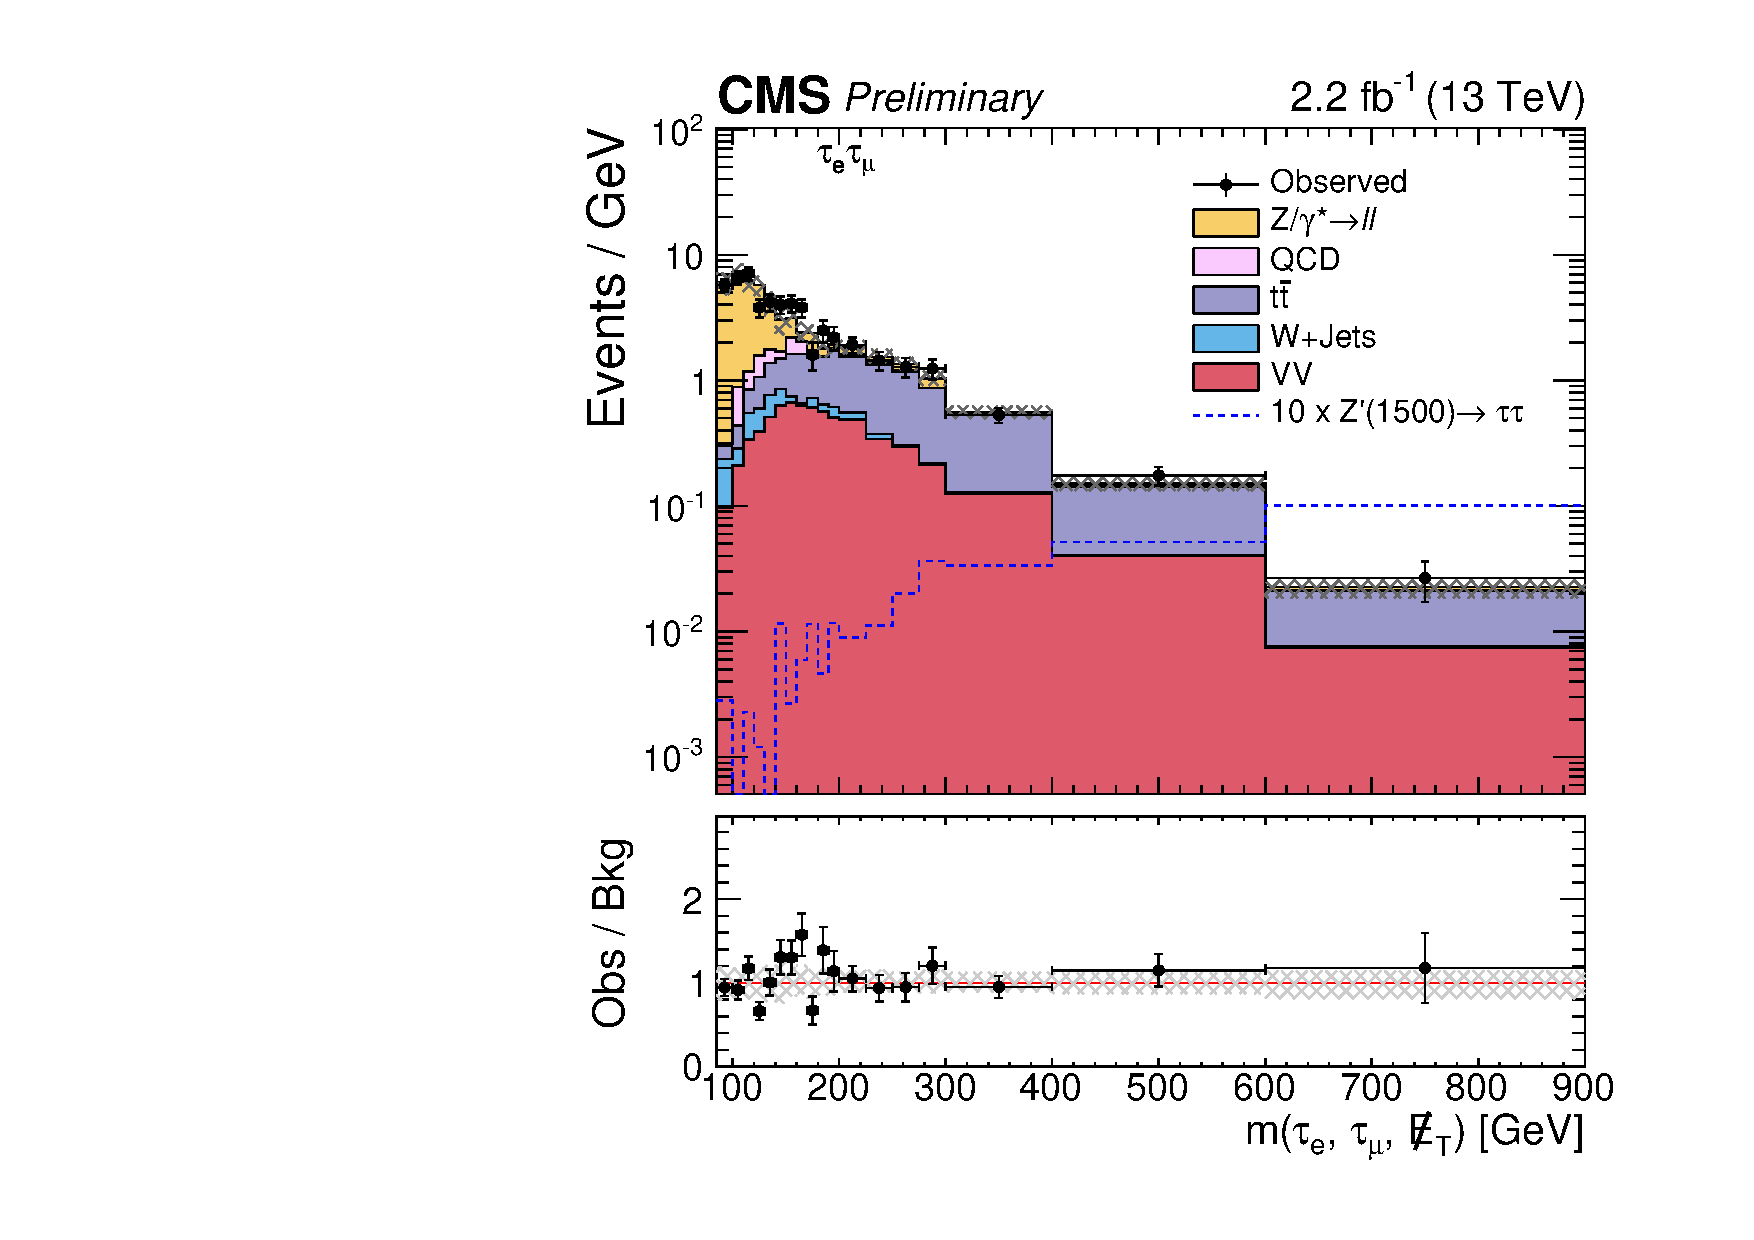
\includegraphics[width=0.45\textwidth]{figures/bkgTemplate_ZPrime1500_em} \\
  \includegraphics[width=0.45\textwidth]{figures/et-em/kinematicDistributions_unblind/em_puweight_OS_signalRegion_mt_e_met}
  \includegraphics[width=0.45\textwidth]{figures/et-em/kinematicDistributions_unblind/em_puweight_OS_signalRegion_mt_mu_met}
  \caption{\label{fig:em_sm_template_and_mt} Top: predicted background
    yields and observed event yields in the \tetm channel after signal
    selection.  Bottom: distributions of transverse mass.}
\end{figure}

Distributions of \pt and $\eta$ are shown in Figure~\ref{fig:em_sr_pt_eta}.
\begin{figure}\centering
  \includegraphics[width=0.45\textwidth]{figures/et-em/kinematicDistributions_unblind/em_puweight_OS_signalRegion_ePt}
  \includegraphics[width=0.45\textwidth]{figures/et-em/kinematicDistributions_unblind/em_puweight_OS_signalRegion_eEta} \\
  \includegraphics[width=0.45\textwidth]{figures/et-em/kinematicDistributions_unblind/em_puweight_OS_signalRegion_mPt}
  \includegraphics[width=0.45\textwidth]{figures/et-em/kinematicDistributions_unblind/em_puweight_OS_signalRegion_mEta}
  \caption{\label{fig:em_sr_pt_eta} Distributions, after \tetm final
    selection, of electron \pt (top left), electron pseudo-rapidity
    (top right), muon \pt (bottom left), muon pseudo-rapidity (bottom
    right).}
\end{figure}
